\documentclass{beamer}  
\usepackage{amsmath}
\usepackage{graphicx}
\usepackage{url}
\usepackage{color}

\makeatletter
\def\url@smallurlstyle{%
 \@ifundefined{selectfont}{\def\UrlFont{\sf}}{\def\UrlFont{\footnotesize\ttfamily}}}
\makeatother
\urlstyle{smallurl}

\mode<presentation>
{ \usetheme{Darmstadt} }

\title{Mesh Networking for in Cave Communications}

\institute{Open SDR}
\author{Philip Balister\inst{1} \and
Paul Walko\inst{2}}
\institute{\inst{1} OpenSDR {\tt\tiny philip@opensdr.com} \and \inst{2} Big Cave Maps {\tt\tiny paul@bigcavemaps.com}}

\date{June 26, 2024}
 
\begin{document} 

\begin{frame}
\titlepage
\end{frame}

\section*{Outline}

\begin{frame}
  \tableofcontents
\end{frame}

\section{Background}

\begin{frame}
\frametitle{Current state of the art in cave communciations}

\begin{itemize}
\item United States: Military field phones
\item Europe: Through the earth communications
	\begin{itemize}
	\item Low frequency (below 500 kHz)
	\item Heyphone: voice only
	\item Cavelink: text only
	\item Both are not available at the moment
	\end{itemize}
\item \tiny\url{https://caverescue.eu/documents/communication/communications-catalogue/}
\item \tiny\url{https://radiolocation.weebly.com/}
\end{itemize}

\end{frame}

\begin{frame}
\frametitle{Operational Challenges}

\begin{itemize}
	\item Existing wired and wireless systems are point to point
	\item Military field phones are purchased from the surplus market
	\item Wireless solutions have large antennas
	\item Prototype solutions exist, but ruggedized packaging is challenging
\end{itemize}

\end{frame}

\begin{frame}
\frametitle{Underground Wireless Networks}

\begin{itemize}
	\item APRS Cave-link, demonstrated in 2013
	\item Sybet SpellCom system
	\item BuecherNet, designed for sensor data
	\item \tiny\url{http://aprs.org/cave-link.html}
	\item \tiny\url{https://sybet.eu/spellcom/}
	\item \tiny\url{https://caves.org/webinars/buechernet-fortstanton-nm/}
\end{itemize}
\end{frame}

\section{Meshtastic}

\begin{frame}
\frametitle{Meshtastic}

\begin{center}
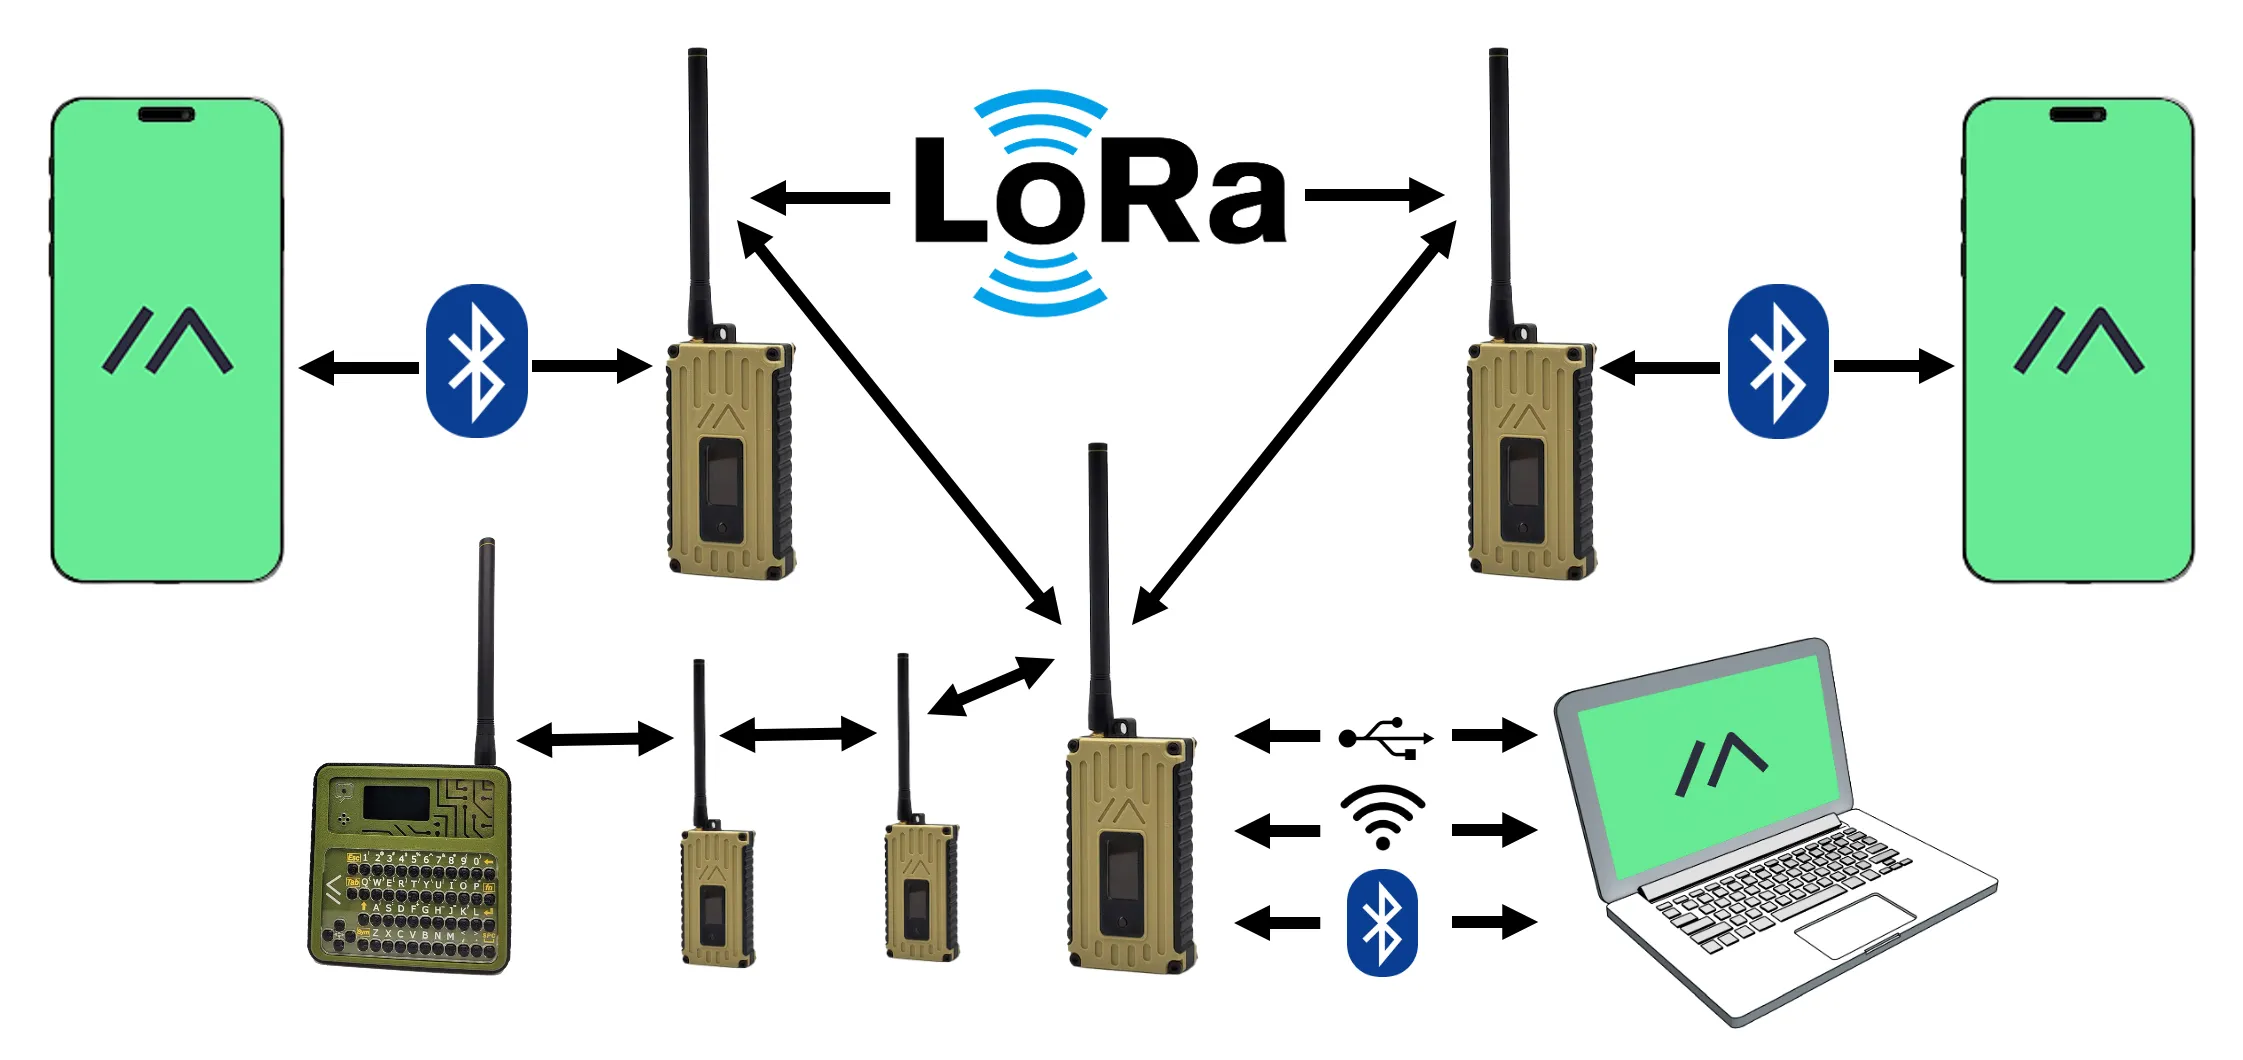
\includegraphics[width=4.0in]{../images/lora-topology-2.png}
\end{center}

\end{frame}


\begin{frame}

\frametitle{Meshtastic Operation}

\begin{itemize}
\item Designed to flood the mesh and assumes multiple routes available
\item When a packet is retransmitted, the hop limit is decremented
\item An node does not retransmit a packet it has heard before
\item A packet is considered acknowledged when the sending node receives it
\item Typical hop limit is set to 3, maximum of 7
\item Nodes check if the channel is busy before transmitting
\item The weaker the received packet is, the sooner a node retransmits it
\end{itemize}

\end{frame}

\begin{frame}
\frametitle{Node Construction}

\begin{center}
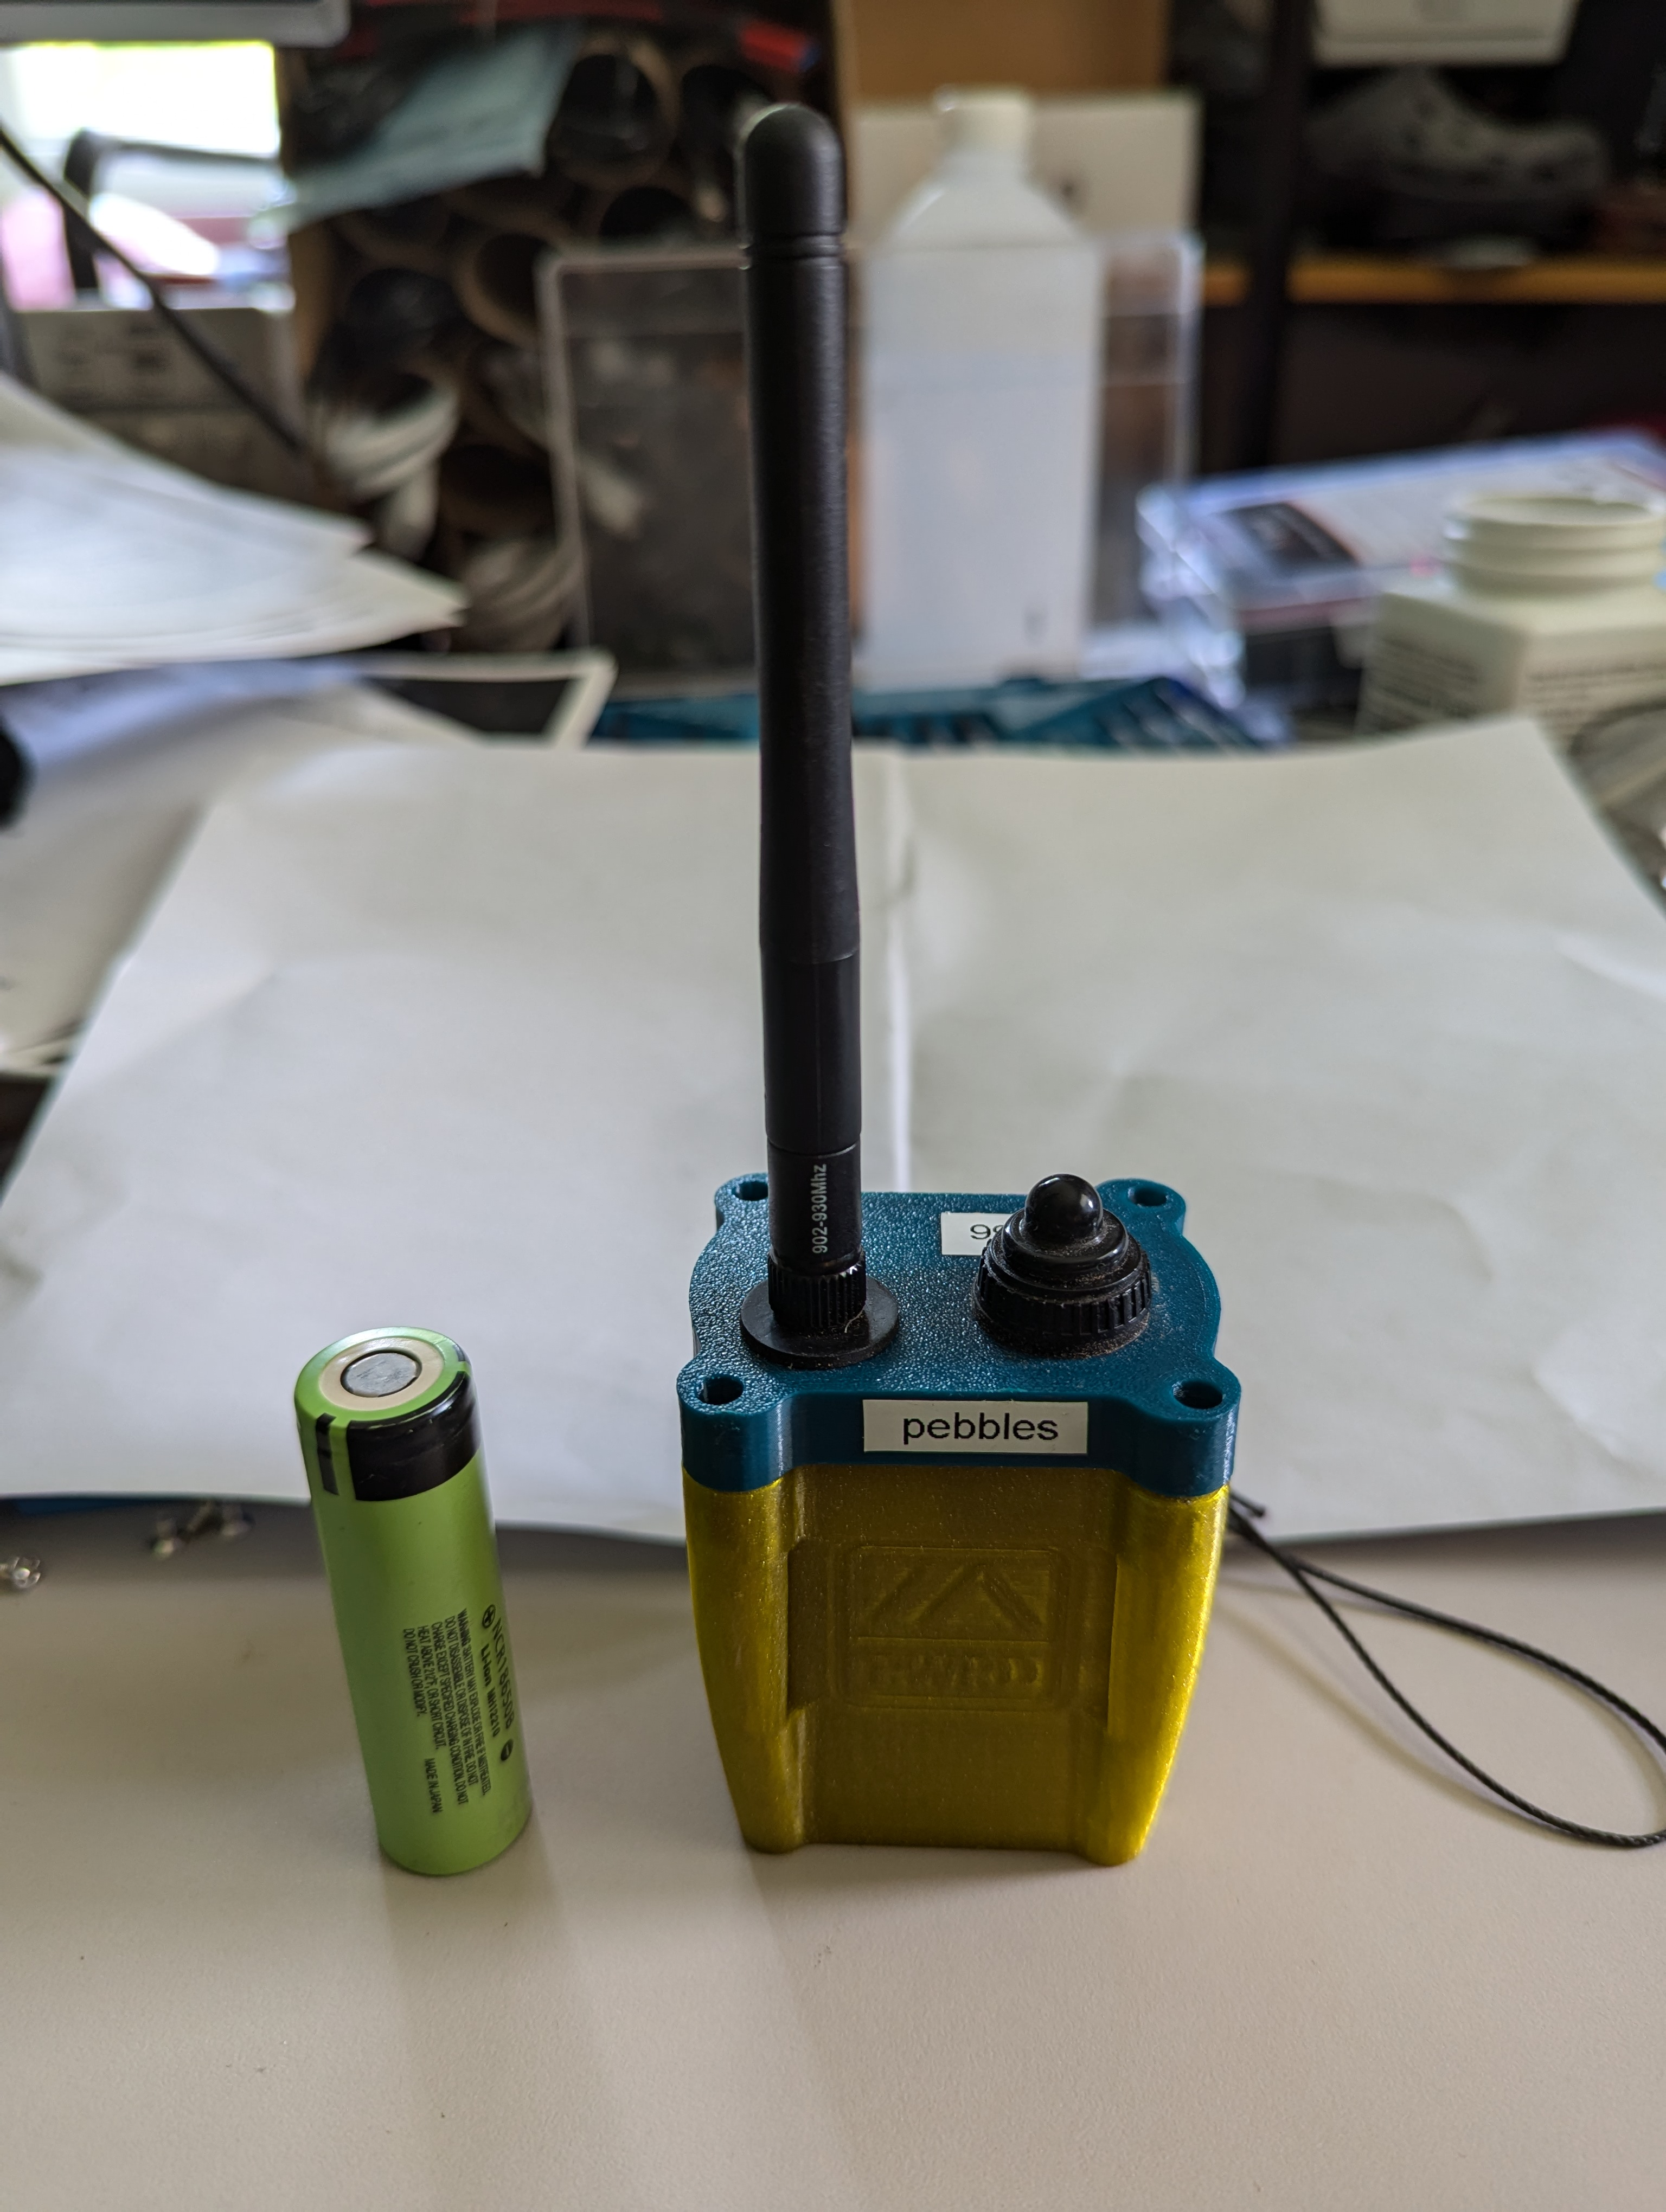
\includegraphics[width=.47\textwidth]{../images/PXL_20240621_162728283.jpg}\hfill
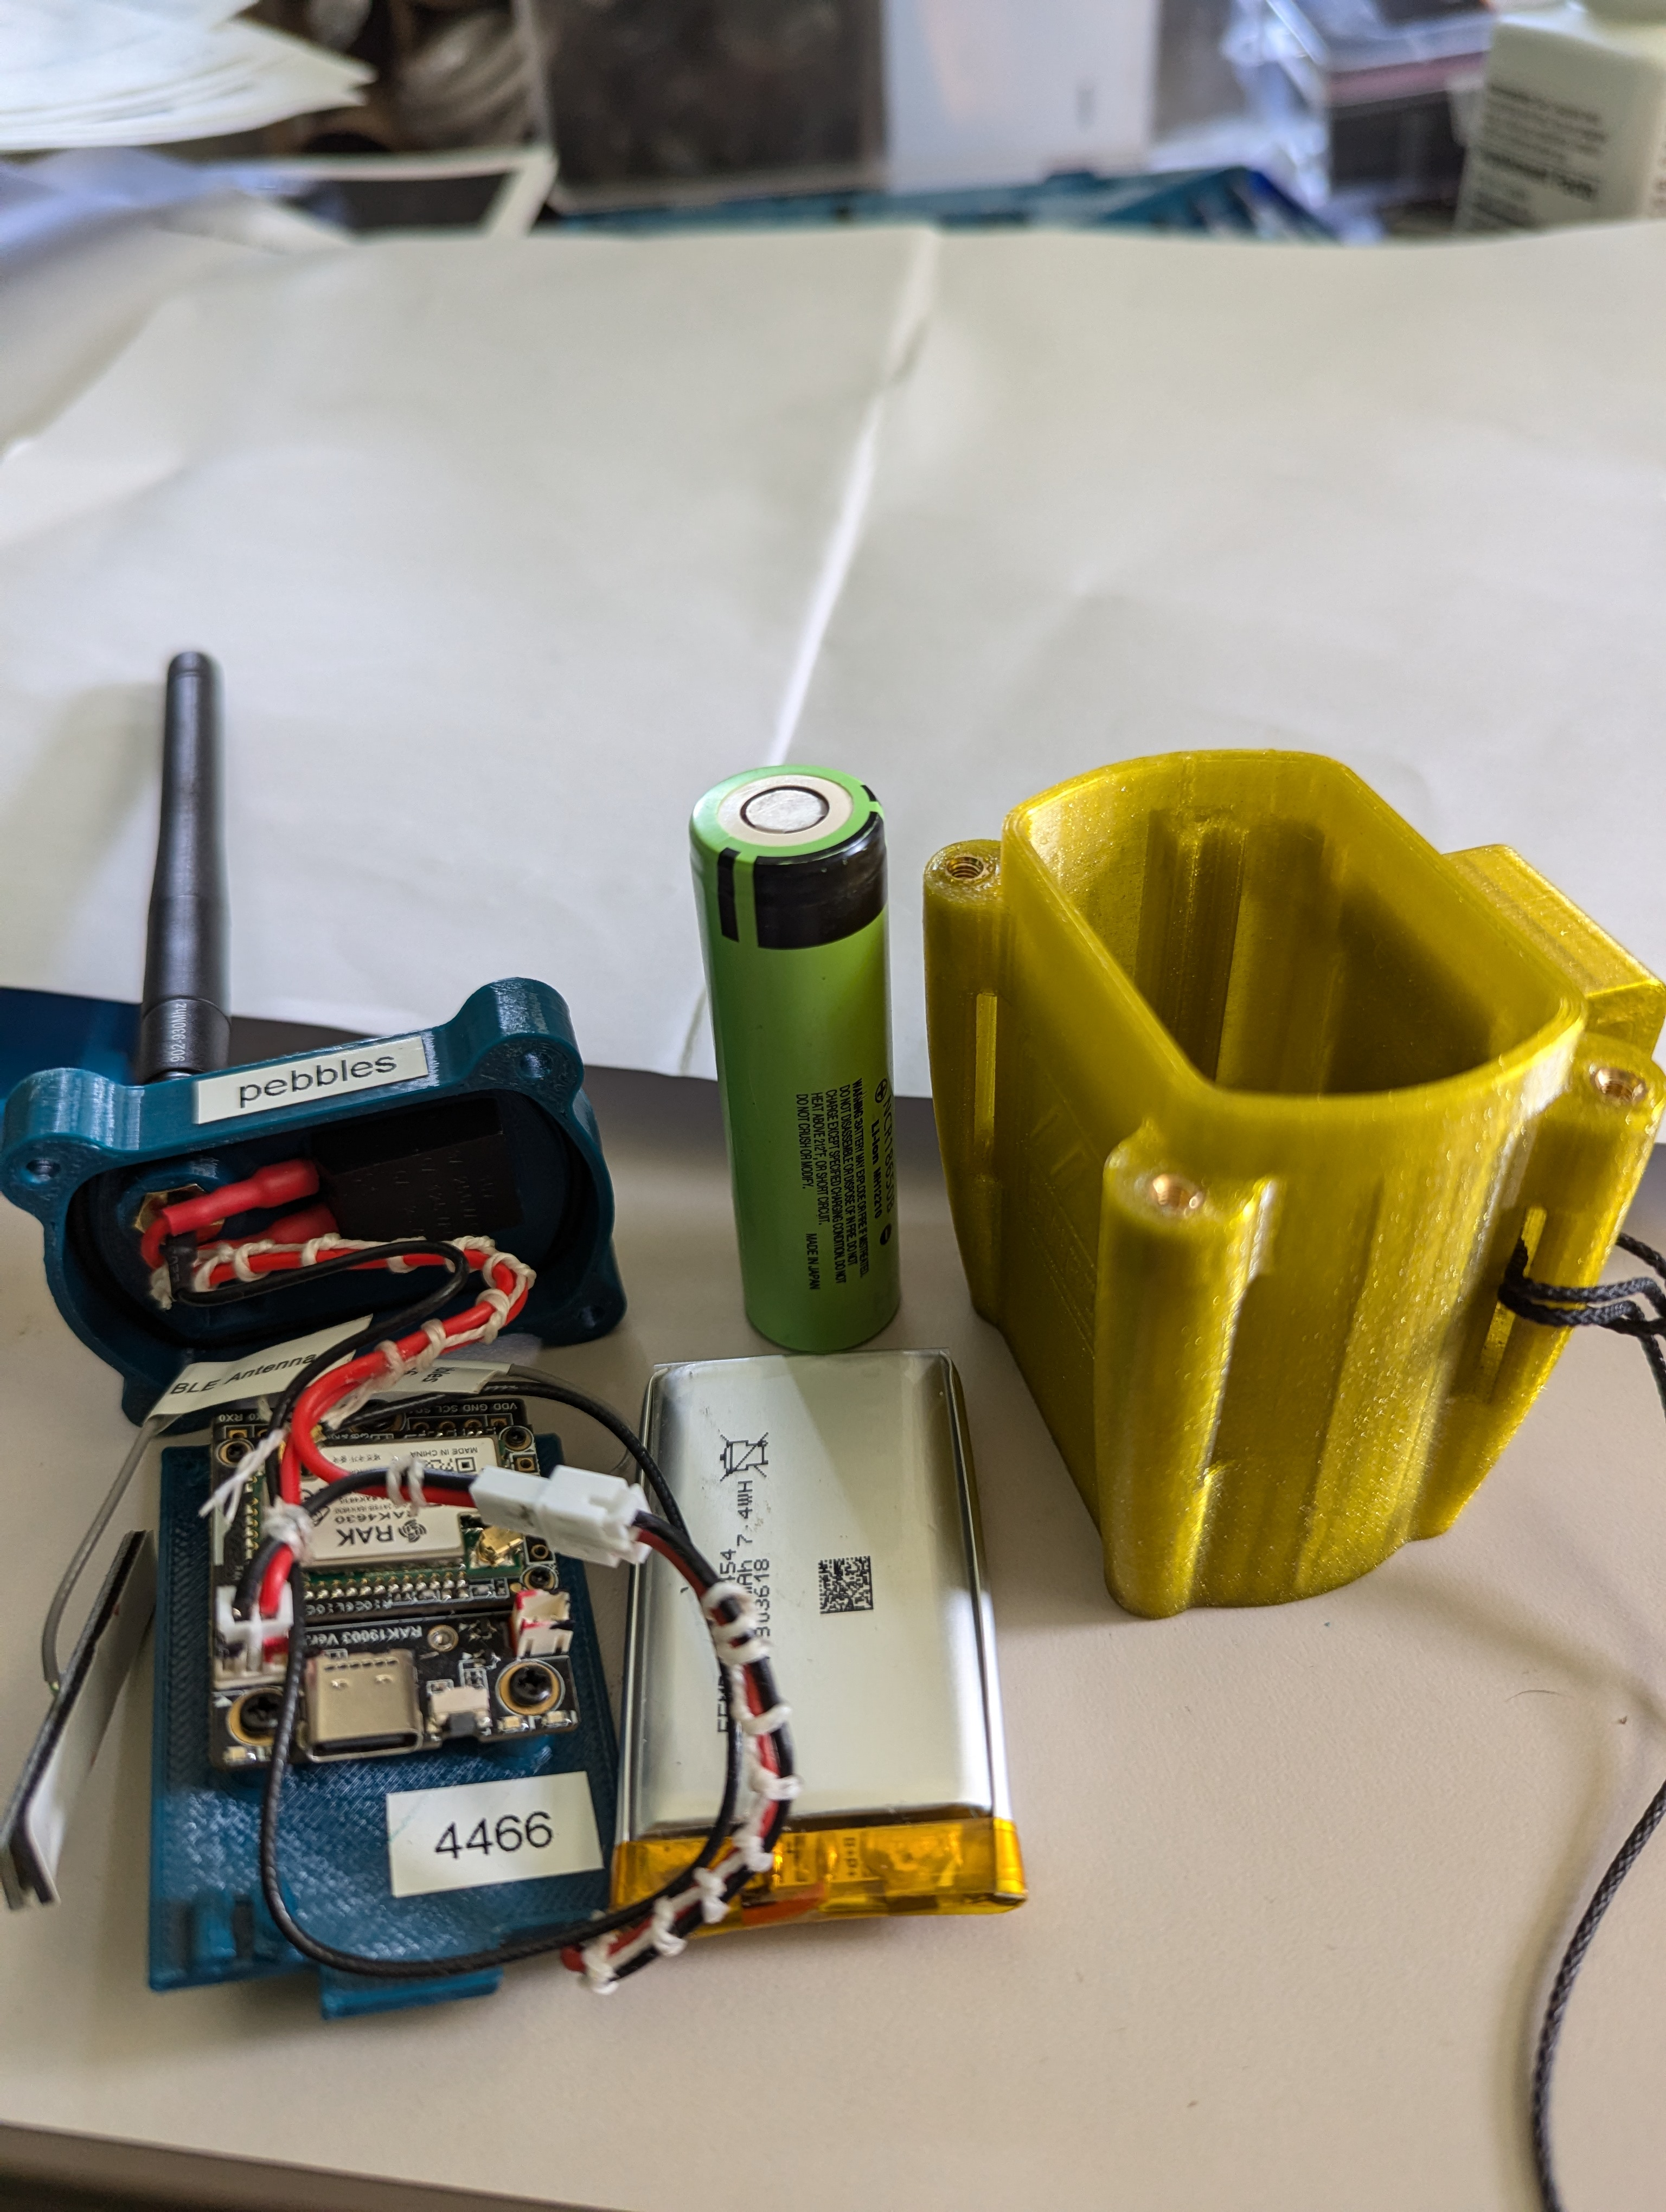
\includegraphics[width=.47\textwidth]{../images/PXL_20240621_162803934.jpg}
\end{center}

\end{frame}

\section{In Cave Testing}

\begin{frame}
\frametitle{Nodes In Cave}

\begin{center}
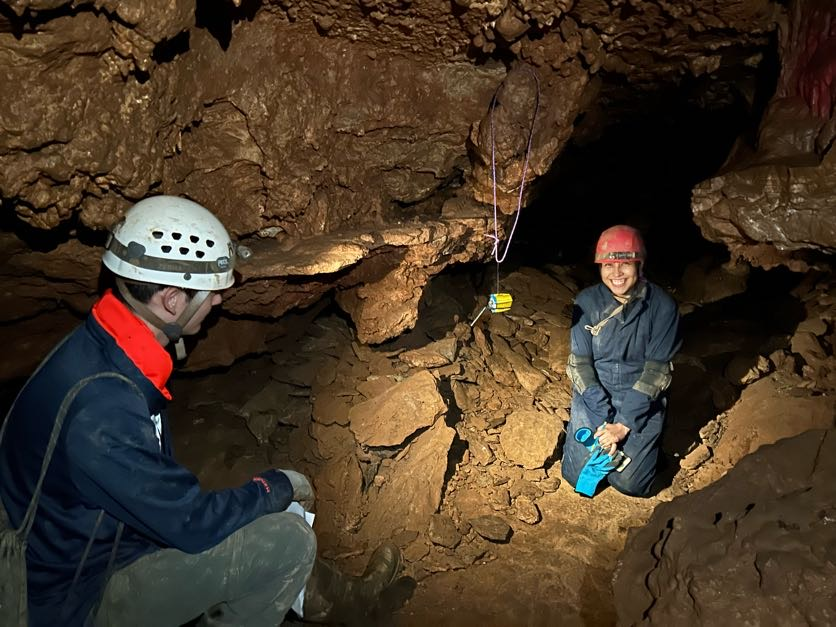
\includegraphics[width=.47\textwidth]{../images/IMG_5732.jpg}\hfill
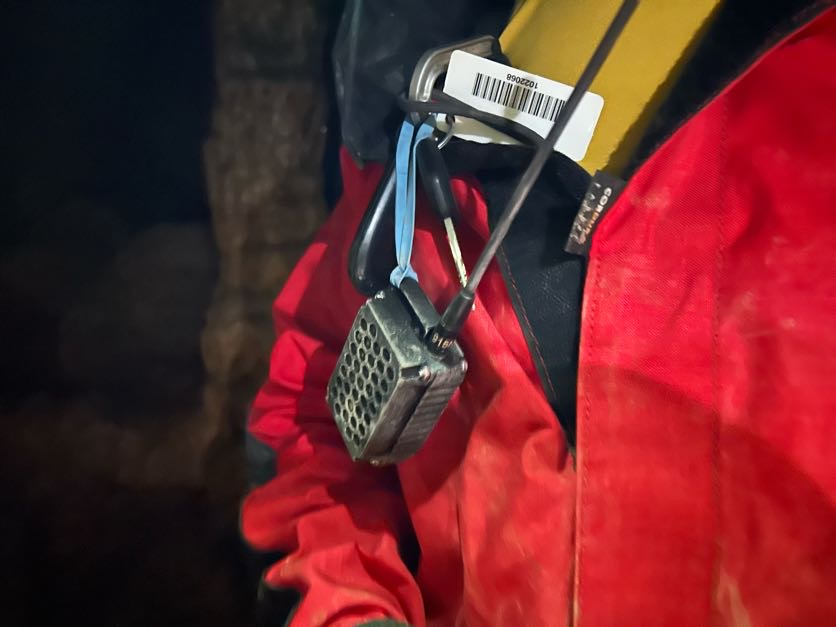
\includegraphics[width=.47\textwidth]{../images/IMG_5751.jpg}
\end{center}

\end{frame}

\begin{frame}
\frametitle{Node Placement}

\begin{center}
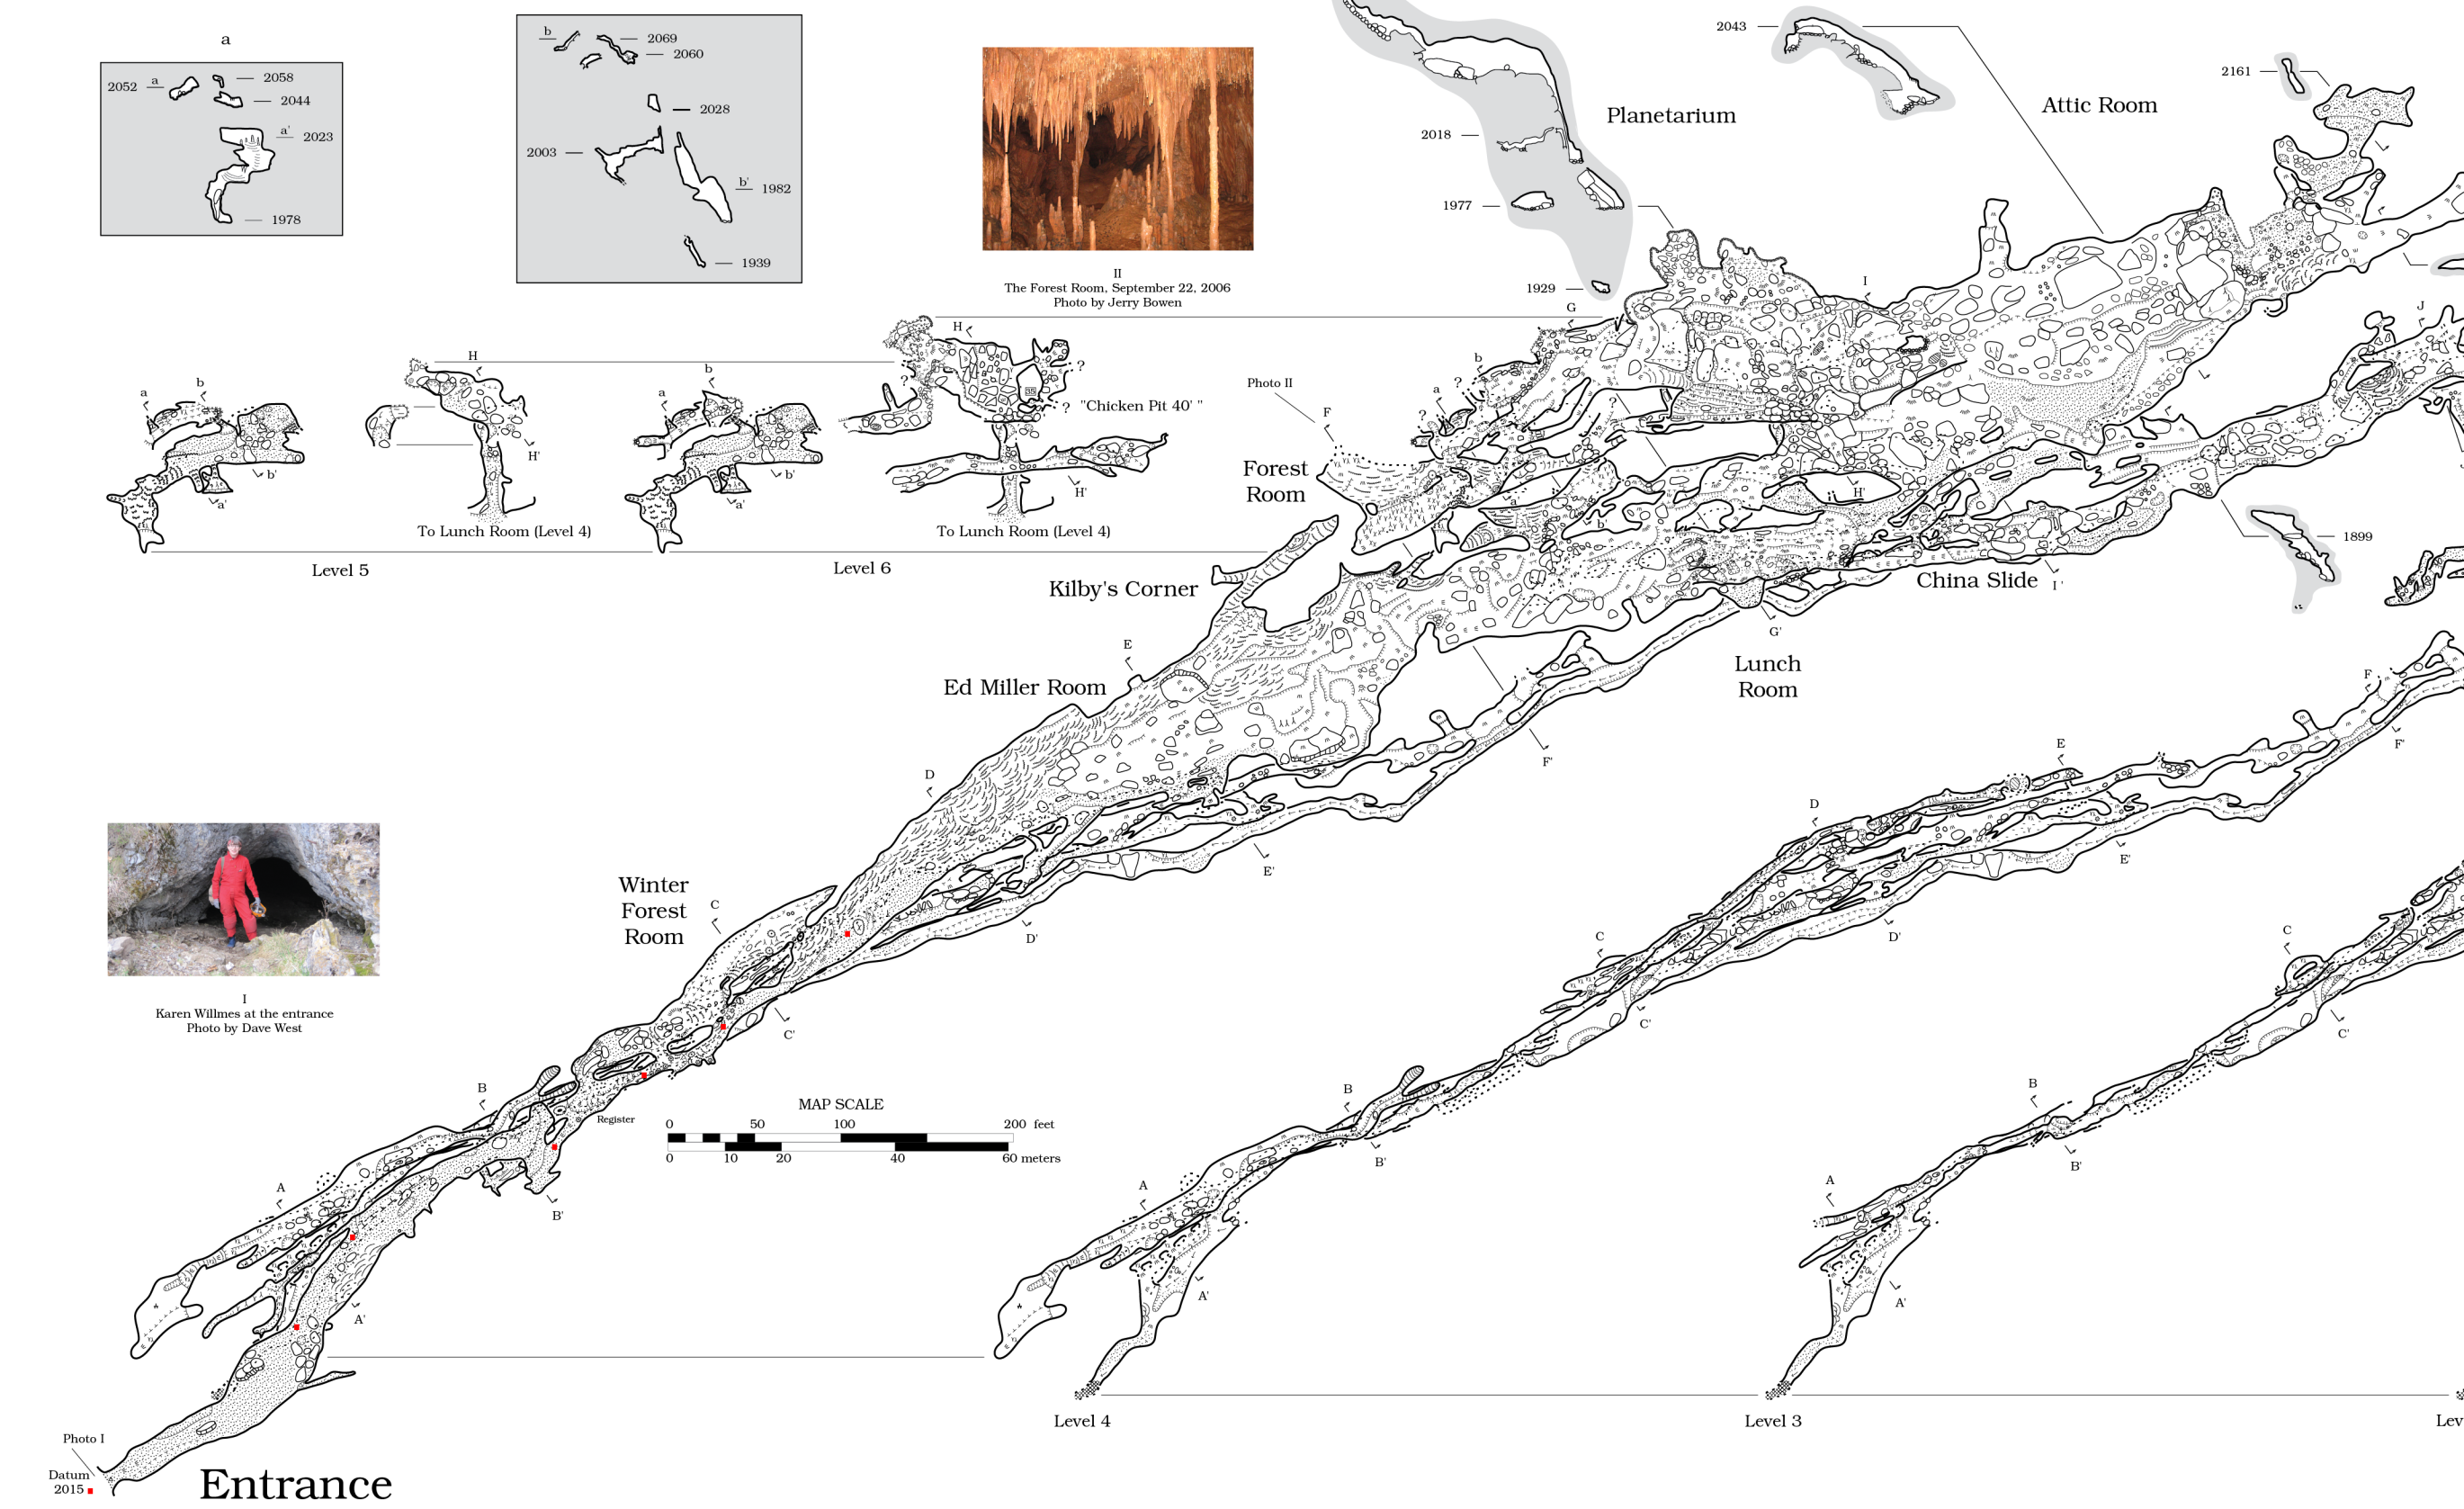
\includegraphics[width=4.0in]{../images/New-River-June-4-2024.png}
\end{center}

\end{frame}

\section{Results}

\begin{frame}

\frametitle{Observations}

\begin{itemize}
\item We can communicate slightly past line of sight
\item Bluetooth is fiddly
\item Optimal node placement is hard
\item Practice is critical
\item Communicators should carry a node
\item Feels like we drop packets due to collisions
\end{itemize}

\end{frame}

\section{Where next?}

\begin{frame}
\frametitle{Future Work}

\begin{itemize}
\item Test zero decrement hop count modification
\item Add a neighbor based packet ack algorithm
\item Conduct longer tests, more nodes
\item Collect all logs from nodes and analyze
\item More field tests, test in an actual mock rescue
\end{itemize}

\end{frame}


\begin{frame}
\frametitle{Conclusions}

\begin{itemize}
\item Promising technology
\item Some development required
\item Using existing technology prevent reinventing a lot of wheels
\end{itemize}
\end{frame}

\begin{frame}
\frametitle{Questions}

Answer my Questions!

\end{frame}

\begin{frame}
\frametitle{Thanks}

\begin{itemize}
\item Richard Cobb - 3D printing of cases
\item Gracie Cornish - In cave photos
\end{itemize}

\end{frame}

\end{document}
